\documentclass[border=5pt]{standalone}
\usepackage{fontspec}
\setmainfont{Times New Roman}
\setmonofont{Courier New}
\usepackage{amsmath,graphicx}
% Shared by the report and the standalone code figure generators.
\usepackage{xcolor,listings}

\definecolor{codeKeyword}{HTML}{174EA6}
\definecolor{codeBuiltin}{HTML}{6F3296}
\definecolor{codeIdentifier}{HTML}{243B53}
\definecolor{codeString}{HTML}{9C3328}
\definecolor{codeComment}{HTML}{396B45}
\definecolor{codeAddition}{HTML}{246B35}
\definecolor{codeDeletion}{HTML}{A12E2E}
\definecolor{codeDiffHeader}{HTML}{176B7D}

\lstdefinestyle{report-code}{
  basicstyle=\ttfamily,
  keywordstyle=\color{codeKeyword},
  keywordstyle=[2]\color{codeBuiltin},
  commentstyle=\color{codeComment},
  stringstyle=\color{codeString},
  identifierstyle=\color{codeIdentifier},
  columns=fullflexible,
  keepspaces=true,
  showspaces=false,
  showstringspaces=false,
  showtabs=false,
  upquote=true,
  tabsize=4,
  numbers=none,
  breaklines=false,
  aboveskip=0pt,
  belowskip=0pt,
  nolol=true
}

\lstdefinestyle{report-python}{
  style=report-code,
  language=[3]Python
}

\lstdefinestyle{report-bash}{
  style=report-code,
  language=bash,
  morekeywords={git}
}

\lstdefinelanguage{ReportDiff}{
  morekeywords={diff,index,git},
  moredelim=[l][\color{codeAddition}]{+},
  moredelim=[l][\color{codeDeletion}]{-},
  moredelim=[l][\color{codeDiffHeader}]{@@}
}
\lstdefinestyle{report-diff}{
  style=report-code,
  language=ReportDiff
}

\setlength{\fboxsep}{7pt}
\setlength{\fboxrule}{0.5pt}
\begin{document}
\begin{minipage}{510pt}
\fontsize{10}{12}\selectfont
\begin{minipage}[t]{506pt}
\vspace{0pt}\textbf{Python: explicit component interfaces}\par\smallskip
\begin{lstlisting}[style=report-python,basicstyle=\ttfamily\fontsize{8}{10.24}\selectfont]
battery.series_count = 1
battery.cell_nominal_voltage = 3.7
converter.input_voltage = battery.nominal_voltage
converter.output_voltage = active.on.voltage
eps.bus_voltage.available = converter.output_voltage
eps.bus_voltage.required = active.on.voltage
\end{lstlisting}
\end{minipage}\par\medskip\begin{minipage}[t]{506pt}
\vspace{0pt}\textbf{GUI: converter input before the battery edit}\par\smallskip
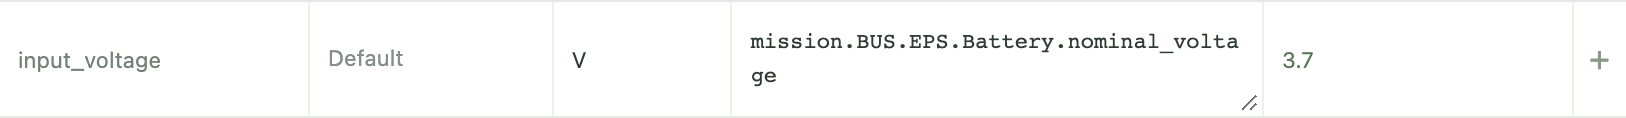
\includegraphics[width=506pt]{interface-before.png}\end{minipage}\par\medskip\begin{minipage}[t]{506pt}
\vspace{0pt}\textbf{GUI: converter input after the battery edit}\par\smallskip
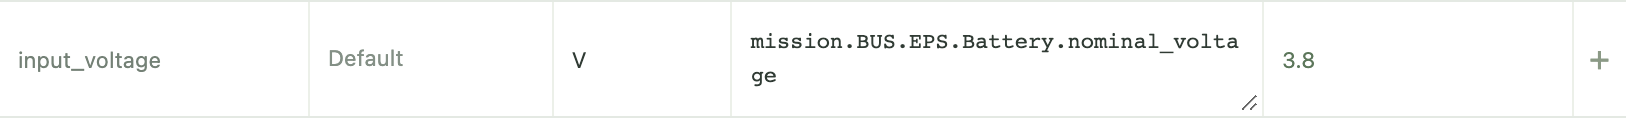
\includegraphics[width=506pt]{interface-after.png}\end{minipage}
\end{minipage}
\end{document}
